\documentclass[10pt]{article}\usepackage[margin=.65in]{geometry}\usepackage[T1]{fontenc}\usepackage{graphicx}\setlength{\parindent}{0pt}\setlength{\parskip}{7pt}\sloppy\begin{document}{\large Stored input extraction to fast polynomial calls}\par The producer completed five main declarations, seven fixed controls and twelve separate named axiom readbacks. Actual stored-array coefficients now supply the existing fast polynomial-call endpoint, with coefficient identities and residual hypotheses derived from the explicit stored contract. Independent source-fidelity review is pending; this archive performs no new proof execution.\par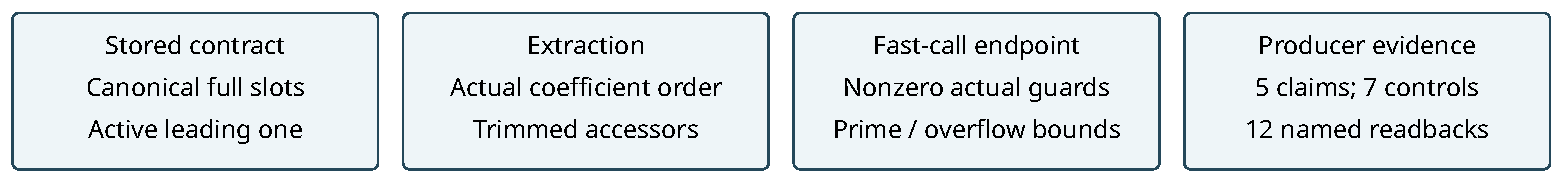
\includegraphics[width=\linewidth]{diagram.pdf}\par Stored assumptions. WellFormed requires degree at most two, U/V capacities three/two, canonical coefficients in every slot, active U slot equal to one, and residual divisibility of decoded accessor polynomials. Nonzero inactive padding is allowed; zero padding is not an assumption. The model extracts actual low coefficients in native qa,ra,sa,ta,qb,rb,sb,tb order. Total getD accesses are used only after capacities are established. Accessor shape handles degrees zero, one and two and uses actual ordinate trimming.

Derived endpoint. stored\_inputs derives support nonemptiness, decoded degree equal to stored degree and the stated Mumford validity under prime p$>$1. degree\_two\_inputs derives canonical fast inputs, support and trimmed-ordinate identities, and both support residual divisibilities. stored\_fast\_calls then returns successful modeled exact quotient/remainder equations, canonical normalized outputs, support length three with leading one, ordinate length at most two and decoded validity. Its assumptions include prime 2$<$p$<$2\textasciicircum{}31, canonical degree-five f, degree-two WellFormed inputs and actual nonzero norm/s1 guards. The native correspondence is the n=1/no-table branch; Field::validate itself admits odd p$>$=5.

Checks and failures. All five successful module receipts and twelve axiom readbacks passed with unchanged bound inputs; the false theorem was rejected with exit 1. Seven controls cover inactive nonzero padding, degree-one/two ordinate trimming, malformed shape/leading coefficient/degree, literal extraction and guards, p17 input validity and full modeled fast-call composition. The fixture uses A=(U[0,0,1],V[1,0]) and B=(U[1,0,1],V[1,1]), with f=[1,0,0,16,16,1]. Outputs are existential kernel-checked lists, not measured Rust trajectories. Two failed construction attempts remain: a rewritten equality, and control errors involving a redundant tactic, missing decidable equality instance, wrong B ordinate and wrong namespace. Final controls use the corrected explicit fixture.

Source provenance. The immutable native snapshot is e62d035ab852be5bbfd27bbe8f11c8f6bfe25f2e, SHA256 26e99b56dace8f848d055e8709bb989622e4caea65aec26d63e00805153dc3c6. The first harness bound live native source, then switched to the pinned snapshot before subsequent work while the shared worktree was merging; no binding failure occurred. Receipts preserve this distinction. Source basis is the native constructor/accessors, validity and addition code, plus existing trim, degree and fast-call constructions. No new method claim is made.

Review boundary and next joint. Compiler/dependency caches were reused and bound. No independent kernel checker or independent source review is included. The prospective review plan calls for source inspection, fresh named-module replay and adversarial checks of padding, leading coefficient, coefficient order, guard domains and trimmed ordinates. Whole dispatch composition and stored validity wrapper follow this component. Physical copying, compiler/counter behavior and class semantics are outside this result. No cohort, timing, runtime qualification or cost claim changes. The diagram is a proof-dependency diagram; canonical scientific graphs are unchanged.
\end{document}